% questions.tex —— 2002 年·全国新课程卷·理科 · 题目内容片段（无答案）
% 由 tools/generate_projects.py 依来源总账自 2002/2002_数学真题_全国新课程理_试题.md 生成，勿手改（改源 MD 后重跑）


\gkpart{数学}

\begin{gktip}
\textbf{来源说明}：本题面依据固定源 PDF 两页 A3 题面逐题转录，原卷印刷页码 114–115。固定源不附答案，答案和解析均由本库独立复算。

\textbf{图形说明}：第 18 题的原卷图形关系重绘为 TikZ/PGFPlots 矢量图。图形标记所指的 PNG 不随仓库保存。
\end{gktip}

\gkpart{一、选择题}

\begin{question}
\gkti{1}曲线

\nopagebreak[4]
\[
\begin{cases}
x=\cos\theta,\\
y=\sin\theta
\end{cases}
\qquad(\theta\text{ \text{为参数}})
\]

上的点到两坐标轴的距离之和的最大值是\mbox{（　　）}

（A）$\dfrac12$　　（B）$\dfrac{\sqrt2}{2}$　　（C）$1$　　（D）$\sqrt2$

\end{question}
\begin{question}
\gkti{2}复数

\nopagebreak[4]
\[
\left(\frac12+\frac{\sqrt3}{2}i\right)^3
\]

的值是\mbox{（　　）}

（A）$-i$　　（B）$i$　　（C）$-1$　　（D）$1$

\end{question}
\begin{question}
\gkti{3}已知 $m\text{、}n$ 为异面直线，$m\subset$ 平面 $\alpha$，$n\subset$ 平面 $\beta$，$\alpha\cap\beta=l$，则 $l$\mbox{（　　）}

（A）与 $m\text{、}n$ 都相交

（B）与 $m\text{、}n$ 中至少一条相交

（C）与 $m\text{、}n$ 都不相交

（D）至多与 $m\text{、}n$ 中的一条相交

\end{question}
\begin{question}
\gkti{4}不等式 $(1+x)(1-|x|)>0$ 的解集是\mbox{（　　）}

（A）$\{x\mid 0\leqslant x<1\}$

（B）$\{x\mid x<0\text{ \text{且} }x\neq-1\}$

（C）$\{x\mid -1<x<1\}$

（D）$\{x\mid x<1\text{ \text{且} }x\neq-1\}$

\end{question}
\begin{question}
\gkti{5}在 $(0,2\pi)$ 内，使 $\sin x>\cos x$ 成立的 $x$ 的取值范围是\mbox{（　　）}

（A）$\left(\dfrac\pi4,\dfrac\pi2\right)\cup\left(\pi,\dfrac{5\pi}4\right)$

（B）$\left(\dfrac\pi4,\pi\right)$

（C）$\left(\dfrac\pi4,\dfrac{5\pi}4\right)$

（D）$\left(\dfrac\pi4,\pi\right)\cup\left(\dfrac{5\pi}4,\dfrac{3\pi}2\right)$

\end{question}
\begin{question}
\gkti{6}设集合

\nopagebreak[4]
\[
M=\left\{x\middle|x=\frac{k}{2}+\frac14,\ k\in\mathbb Z\right\},\qquad
N=\left\{x\middle|x=\frac{k}{4}+\frac12,\ k\in\mathbb Z\right\},
\]

则\mbox{（　　）}

（A）$M=N$　　（B）$M\subseteq N$　　（C）$M\supseteq N$　　（D）$M\cap N=\varnothing$

\end{question}
\begin{question}
\gkti{7}正六棱柱 $ABCDEF-A_1B_1C_1D_1E_1F_1$ 的底面边长为 1，侧棱长为 $\sqrt2$，则这个棱柱侧面对角线 $E_1D$ 与 $BC_1$ 所成的角是\mbox{（　　）}

（A）$90^\circ$　　（B）$60^\circ$　　（C）$45^\circ$　　（D）$30^\circ$

\end{question}
\begin{question}
\gkti{8}函数 $y=x^2+bx+c$，$x\in[0,+\infty)$ 是单调函数的充要条件是\mbox{（　　）}

（A）$b\geqslant0$　　（B）$b\leqslant0$　　（C）$b>0$　　（D）$b<0$

\end{question}
\begin{question}
\gkti{9}已知 $0<x<y<a<1$，则有\mbox{（　　）}

（A）$\log_a(xy)<0$

（B）$0<\log_a(xy)<1$

（C）$1<\log_a(xy)<2$

（D）$\log_a(xy)>2$

\end{question}
\begin{question}
\gkti{10}平面直角坐标系中，$O$ 为坐标原点，已知两点 $A(3,1)\text{、}B(-1,3)$，若点 $C$ 满足

\nopagebreak[4]
\[
\overrightarrow{OC}=\alpha\overrightarrow{OA}+\beta\overrightarrow{OB},
\qquad \alpha,\beta\in\mathbb R,\quad \alpha+\beta=1,
\]

则点 $C$ 的轨迹方程为\mbox{（　　）}

（A）$3x+2y-11=0$

（B）$(x-1)^2+(y-2)^2=5$

（C）$2x-y=0$

（D）$x+2y-5=0$

\end{question}
\begin{question}
\gkti{11}从正方体的 6 个面中选取 3 个面，其中有 2 个面不相邻的选法共有\mbox{（　　）}

（A）8 种　　（B）12 种　　（C）16 种　　（D）20 种

\end{question}
\begin{question}
\gkti{12}据 2002 年 3 月 5 日九届人大五次会议《政府工作报告》：“2001 年国内生产总值达到 95933 亿元，比上年增长 7.3\%”，如果“十五”期间（2001 年—2005 年）每年的国内生产总值都按此年增长率增长，那么到“十五”末我国国内年生产总值约为\mbox{（　　）}

（A）115000 亿元　　（B）120000 亿元　　（C）127000 亿元　　（D）135000 亿元

\end{question}
\gkpart{二、填空题}

\begin{question}
\gkti{13}函数

\nopagebreak[4]
\[
y=\frac{2x}{1+x},\qquad x\in(-1,+\infty)
\]

图象与其反函数图象的交点为\gkblank{}。

\end{question}
\begin{question}
\gkti{14}椭圆 $5x^2+ky^2=5$ 的一个焦点是 $(0,2)$，那么 $k=$\gkblank{}。

\end{question}
\begin{question}
\gkti{15}直线 $x=0\text{、}y=0\text{、}x=2$ 与曲线 $y=(\sqrt2)^x$ 所围成的图形绕 $x$ 轴旋转一周而成的旋转体的体积等于\gkblank{}。

\end{question}
\begin{question}
\gkti{16}已知 $f(x)=\dfrac{x^2}{1+x^2}$，那么

\nopagebreak[4]
\[
f(1)+f(2)+f\left(\frac12\right)+f(3)+f\left(\frac13\right)+f(4)+f\left(\frac14\right)=\_\_\_\_\_\_
\]

。

\end{question}
\gkpart{三、解答题}

\begin{question}
\gkti{17}已知 $\cos\left(\alpha+\dfrac\pi4\right)=\dfrac35$，$\dfrac\pi2\leqslant\alpha<\dfrac{3\pi}2$，求 $\cos\left(2\alpha+\dfrac\pi4\right)$ 的值。

\Needspace{0.4\textheight}
\end{question}
\begin{question}
\gkti{18}【甲】正三棱柱 $ABC-A_1B_1C_1$ 的底面边长为 $a$，侧棱长为 $\sqrt2a$。
\nopagebreak[4]
\begin{center}% 2002 年全国新课程理科第 18 题甲：正三棱柱
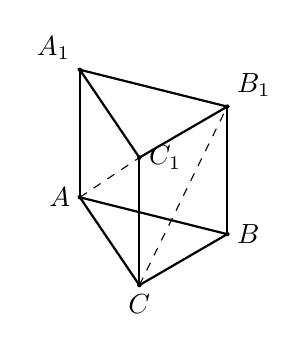
\begin{tikzpicture}[>=stealth,scale=0.72]
  \coordinate (A) at (0,0);
  \coordinate (B) at (2.6,-0.65);
  \coordinate (C) at (1.05,-1.55);
  \coordinate (Aone) at (0,2.25);
  \coordinate (Bone) at (2.6,1.60);
  \coordinate (Cone) at (1.05,0.70);
  \draw[thick] (A)--(B)--(C)--cycle;
  \draw[thick] (Aone)--(Bone)--(Cone)--cycle;
  \draw[thick] (A)--(Aone) (B)--(Bone) (C)--(Cone);
  \draw[dashed] (A)--(Cone) (C)--(Bone);
  \fill (A) circle (1.1pt) node[left] {$A$};
  \fill (B) circle (1.1pt) node[right] {$B$};
  \fill (C) circle (1.1pt) node[below] {$C$};
  \fill (Aone) circle (1.1pt) node[above left] {$A_1$};
  \fill (Bone) circle (1.1pt) node[above right] {$B_1$};
  \fill (Cone) circle (1.1pt) node[right] {$C_1$};
\end{tikzpicture}
\end{center}
\nopagebreak[4]
（1） 建立适当的坐标系，并写出点 $A\text{、}B\text{、}A_1\text{、}C_1$ 的坐标；

（2） 求 $AC_1$ 与侧面 $ABB_1A_1$ 所成的角。

【乙】如图，正方形 $ABCD\text{、}ABEF$ 的边长都是 1，而且平面 $ABCD\text{、}ABEF$ 互相垂直。点 $M$ 在 $AC$ 上移动，点 $N$ 在 $BF$ 上移动，若 $CM=BN=a$（$0<a<\sqrt2$）。
\nopagebreak[4]
\begin{center}% 2002 年全国新课程理科第 18 题乙：两个互相垂直的正方形
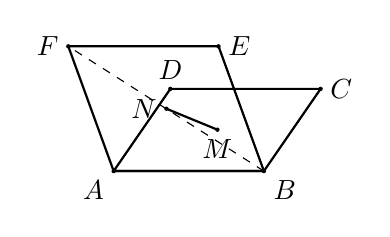
\begin{tikzpicture}[>=stealth,scale=0.72]
  \coordinate (A) at (0,0);
  \coordinate (B) at (2.65,0);
  \coordinate (C) at (3.65,1.45);
  \coordinate (D) at (1.0,1.45);
  \coordinate (E) at (1.85,2.20);
  \coordinate (F) at (-0.80,2.20);
  \coordinate (M) at (1.83,0.73);
  \coordinate (N) at (0.93,1.10);
  \draw[thick] (A)--(B)--(C)--(D)--cycle;
  \draw[thick] (A)--(B)--(E)--(F)--cycle;
  \draw[dashed] (A)--(D) (B)--(F);
  \draw[thick] (M)--(N);
  \fill (A) circle (1.1pt) node[below left] {$A$};
  \fill (B) circle (1.1pt) node[below right] {$B$};
  \fill (C) circle (1.1pt) node[right] {$C$};
  \fill (D) circle (1.1pt) node[above] {$D$};
  \fill (E) circle (1.1pt) node[right] {$E$};
  \fill (F) circle (1.1pt) node[left] {$F$};
  \fill (M) circle (1.1pt) node[below] {$M$};
  \fill (N) circle (1.1pt) node[left] {$N$};
\end{tikzpicture}
\end{center}
\nopagebreak[4]
（1） 求 $MN$ 的长；

（2） $a$ 为何值时，$MN$ 的长最小；

（3） 当 $MN$ 的长最小时，求面 $MNA$ 与面 $MNB$ 所成二面角 $\alpha$ 的大小。

\end{question}
\begin{question}
\gkti{19}某单位 6 个员工借助互联网开展工作，每个员工上网的概率都是 0.5（相互独立）。

（1） 求至少 3 人同时上网的概率；

（2） 至少几人同时上网的概率小于 0.3？

\end{question}
\begin{question}
\gkti{20}已知 $a>0$，函数

\nopagebreak[4]
\[
f(x)=\frac{1-ax}{x},\qquad x\in(0,+\infty).
\]

设 $0<x_1<\dfrac2a$，记曲线 $y=f(x)$ 在点 $M(x_1,f(x_1))$ 处的切线为 $l$。

（1） 求 $l$ 的方程；

（2） 设 $l$ 与 $x$ 轴交点为 $(x_2,0)$。证明：

① $0<x_2\leqslant\dfrac1a$；

② 若 $x_1<\dfrac1a$，则 $x_1<x_2<\dfrac1a$。

\end{question}
\begin{question}
\gkti{21}已知两点 $M(-1,0)\text{、}N(1,0)$，且点 $P$ 使 $\overrightarrow{MP}\cdot\overrightarrow{MN}$、$\overrightarrow{PM}\cdot\overrightarrow{PN}$、$\overrightarrow{NM}\cdot\overrightarrow{NP}$ 成公差小于零的等差数列。

（1） 点 $P$ 的轨迹是什么曲线？

（2） 若点 $P$ 坐标为 $(x_0,y_0)$，记 $\theta$ 为 $\overrightarrow{PM}$ 与 $\overrightarrow{PN}$ 的夹角，求 $\tan\theta$。

\end{question}
\begin{question}
\gkti{22}已知 $\{a_n\}$ 是由非负整数组成的数列，满足 $a_1=0\text{、}a_2=3$，

\nopagebreak[4]
\[
a_{n+1}a_n=(a_{n-1}+2)(a_{n-2}+2),\qquad n=3,4,5,\cdots.
\]

（1） 求 $a_3$；

（2） 证明 $a_n=a_{n-2}+2$，$n=3,4,5,\cdots$；

（3） 求 $\{a_n\}$ 的通项公式及其前 $n$ 项和 $S_n$。

\end{question}